\documentclass[twoside]{book}

% Packages required by doxygen
\usepackage{fixltx2e}
\usepackage{calc}
\usepackage{doxygen}
\usepackage[export]{adjustbox} % also loads graphicx
\usepackage{graphicx}
\usepackage[utf8]{inputenc}
\usepackage{makeidx}
\usepackage{multicol}
\usepackage{multirow}
\PassOptionsToPackage{warn}{textcomp}
\usepackage{textcomp}
\usepackage[nointegrals]{wasysym}
\usepackage[table]{xcolor}

% Font selection
\usepackage[T1]{fontenc}
\usepackage[scaled=.90]{helvet}
\usepackage{courier}
\usepackage{amssymb}
\usepackage{sectsty}
\renewcommand{\familydefault}{\sfdefault}
\allsectionsfont{%
  \fontseries{bc}\selectfont%
  \color{darkgray}%
}
\renewcommand{\DoxyLabelFont}{%
  \fontseries{bc}\selectfont%
  \color{darkgray}%
}
\newcommand{\+}{\discretionary{\mbox{\scriptsize$\hookleftarrow$}}{}{}}

% Page & text layout
\usepackage{geometry}
\geometry{%
  a4paper,%
  top=2.5cm,%
  bottom=2.5cm,%
  left=2.5cm,%
  right=2.5cm%
}
\tolerance=750
\hfuzz=15pt
\hbadness=750
\setlength{\emergencystretch}{15pt}
\setlength{\parindent}{0cm}
\setlength{\parskip}{0.2cm}
\makeatletter
\renewcommand{\paragraph}{%
  \@startsection{paragraph}{4}{0ex}{-1.0ex}{1.0ex}{%
    \normalfont\normalsize\bfseries\SS@parafont%
  }%
}
\renewcommand{\subparagraph}{%
  \@startsection{subparagraph}{5}{0ex}{-1.0ex}{1.0ex}{%
    \normalfont\normalsize\bfseries\SS@subparafont%
  }%
}
\makeatother

% Headers & footers
\usepackage{fancyhdr}
\pagestyle{fancyplain}
\fancyhead[LE]{\fancyplain{}{\bfseries\thepage}}
\fancyhead[CE]{\fancyplain{}{}}
\fancyhead[RE]{\fancyplain{}{\bfseries\leftmark}}
\fancyhead[LO]{\fancyplain{}{\bfseries\rightmark}}
\fancyhead[CO]{\fancyplain{}{}}
\fancyhead[RO]{\fancyplain{}{\bfseries\thepage}}
\fancyfoot[LE]{\fancyplain{}{}}
\fancyfoot[CE]{\fancyplain{}{}}
\fancyfoot[RE]{\fancyplain{}{\bfseries\scriptsize Generated on Mon Dec 7 2015 20\+:52\+:16 for Bit-\/\+Man! by Doxygen }}
\fancyfoot[LO]{\fancyplain{}{\bfseries\scriptsize Generated on Mon Dec 7 2015 20\+:52\+:16 for Bit-\/\+Man! by Doxygen }}
\fancyfoot[CO]{\fancyplain{}{}}
\fancyfoot[RO]{\fancyplain{}{}}
\renewcommand{\footrulewidth}{0.4pt}
\renewcommand{\chaptermark}[1]{%
  \markboth{#1}{}%
}
\renewcommand{\sectionmark}[1]{%
  \markright{\thesection\ #1}%
}

% Indices & bibliography
\usepackage{natbib}
\usepackage[titles]{tocloft}
\setcounter{tocdepth}{3}
\setcounter{secnumdepth}{5}
\makeindex

% Hyperlinks (required, but should be loaded last)
\usepackage{ifpdf}
\ifpdf
  \usepackage[pdftex,pagebackref=true]{hyperref}
\else
  \usepackage[ps2pdf,pagebackref=true]{hyperref}
\fi
\hypersetup{%
  colorlinks=true,%
  linkcolor=blue,%
  citecolor=blue,%
  unicode%
}

% Custom commands
\newcommand{\clearemptydoublepage}{%
  \newpage{\pagestyle{empty}\cleardoublepage}%
}


%===== C O N T E N T S =====

\begin{document}

% Titlepage & ToC
\hypersetup{pageanchor=false,
             bookmarks=true,
             bookmarksnumbered=true,
             pdfencoding=unicode
            }
\pagenumbering{roman}
\begin{titlepage}
\vspace*{7cm}
\begin{center}%
{\Large Bit-\/\+Man! }\\
\vspace*{1cm}
{\large Generated by Doxygen 1.8.10}\\
\vspace*{0.5cm}
{\small Mon Dec 7 2015 20:52:16}\\
\end{center}
\end{titlepage}
\clearemptydoublepage
\tableofcontents
\clearemptydoublepage
\pagenumbering{arabic}
\hypersetup{pageanchor=true}

%--- Begin generated contents ---
\chapter{Bug List}
\label{bug}
\hypertarget{bug}{}

\begin{DoxyRefList}
\item[\label{bug__bug000001}%
\hypertarget{bug__bug000001}{}%
File \hyperlink{_autowalk_8cs}{Autowalk.cs} ]Collision isn\textquotesingle{}t handled. 
\item[\label{bug__bug000002}%
\hypertarget{bug__bug000002}{}%
File \hyperlink{_character_motor_8cs}{Character\+Motor.cs} ]Accelerates spontaniously if attached to a camera 
\item[\label{bug__bug000003}%
\hypertarget{bug__bug000003}{}%
File \hyperlink{_f_p_s_input_controller_8cs}{F\+P\+S\+Input\+Controller.cs} ]None 
\item[\label{bug__bug000004}%
\hypertarget{bug__bug000004}{}%
File \hyperlink{_load_on_click_8cs}{Load\+On\+Click.cs} ]None
\end{DoxyRefList}
\chapter{Hierarchical Index}
\section{Class Hierarchy}
This inheritance list is sorted roughly, but not completely, alphabetically\+:\begin{DoxyCompactList}
\item \contentsline{section}{Character\+Motor.\+Character\+Motor\+Jumping}{\pageref{class_character_motor_1_1_character_motor_jumping}}{}
\item \contentsline{section}{Character\+Motor.\+Character\+Motor\+Movement}{\pageref{class_character_motor_1_1_character_motor_movement}}{}
\item \contentsline{section}{Character\+Motor.\+Character\+Motor\+Moving\+Platform}{\pageref{class_character_motor_1_1_character_motor_moving_platform}}{}
\item \contentsline{section}{Character\+Motor.\+Character\+Motor\+Sliding}{\pageref{class_character_motor_1_1_character_motor_sliding}}{}
\item Mono\+Behaviour\begin{DoxyCompactList}
\item \contentsline{section}{Autowalk}{\pageref{class_autowalk}}{}
\item \contentsline{section}{Character\+Motor}{\pageref{class_character_motor}}{}
\item \contentsline{section}{F\+P\+S\+Input\+Controller}{\pageref{class_f_p_s_input_controller}}{}
\item \contentsline{section}{Load\+On\+Click}{\pageref{class_load_on_click}}{}
\end{DoxyCompactList}
\end{DoxyCompactList}

\chapter{Class Index}
\section{Class List}
Here are the classes, structs, unions and interfaces with brief descriptions\+:\begin{DoxyCompactList}
\item\contentsline{section}{\hyperlink{class_autowalk}{Autowalk} }{\pageref{class_autowalk}}{}
\item\contentsline{section}{\hyperlink{class_character_motor}{Character\+Motor} }{\pageref{class_character_motor}}{}
\item\contentsline{section}{\hyperlink{class_character_motor_1_1_character_motor_jumping}{Character\+Motor.\+Character\+Motor\+Jumping} }{\pageref{class_character_motor_1_1_character_motor_jumping}}{}
\item\contentsline{section}{\hyperlink{class_character_motor_1_1_character_motor_movement}{Character\+Motor.\+Character\+Motor\+Movement} }{\pageref{class_character_motor_1_1_character_motor_movement}}{}
\item\contentsline{section}{\hyperlink{class_character_motor_1_1_character_motor_moving_platform}{Character\+Motor.\+Character\+Motor\+Moving\+Platform} }{\pageref{class_character_motor_1_1_character_motor_moving_platform}}{}
\item\contentsline{section}{\hyperlink{class_character_motor_1_1_character_motor_sliding}{Character\+Motor.\+Character\+Motor\+Sliding} }{\pageref{class_character_motor_1_1_character_motor_sliding}}{}
\item\contentsline{section}{\hyperlink{class_f_p_s_input_controller}{F\+P\+S\+Input\+Controller} }{\pageref{class_f_p_s_input_controller}}{}
\item\contentsline{section}{\hyperlink{class_load_on_click}{Load\+On\+Click} }{\pageref{class_load_on_click}}{}
\end{DoxyCompactList}

\chapter{File Index}
\section{File List}
Here is a list of all files with brief descriptions\+:\begin{DoxyCompactList}
\item\contentsline{section}{\hyperlink{_autowalk_8cs}{Autowalk.\+cs} \\*This script moves your player automatically in the direction he is looking at }{\pageref{_autowalk_8cs}}{}
\item\contentsline{section}{\hyperlink{_character_motor_8cs}{Character\+Motor.\+cs} \\*Character motor holds all the values for the speed and movement of a 3\+D object within unity and handles collision }{\pageref{_character_motor_8cs}}{}
\item\contentsline{section}{\hyperlink{_f_p_s_input_controller_8cs}{F\+P\+S\+Input\+Controller.\+cs} \\*The controller for the main character that navigates the \hyperlink{class_character_motor}{Character\+Motor} movement properties }{\pageref{_f_p_s_input_controller_8cs}}{}
\item\contentsline{section}{\hyperlink{_load_on_click_8cs}{Load\+On\+Click.\+cs} \\*Class designed to change scenes within the Unity project }{\pageref{_load_on_click_8cs}}{}
\end{DoxyCompactList}

\chapter{Class Documentation}
\hypertarget{class_autowalk}{}\section{Autowalk Class Reference}
\label{class_autowalk}\index{Autowalk@{Autowalk}}
Inheritance diagram for Autowalk\+:\begin{figure}[H]
\begin{center}
\leavevmode
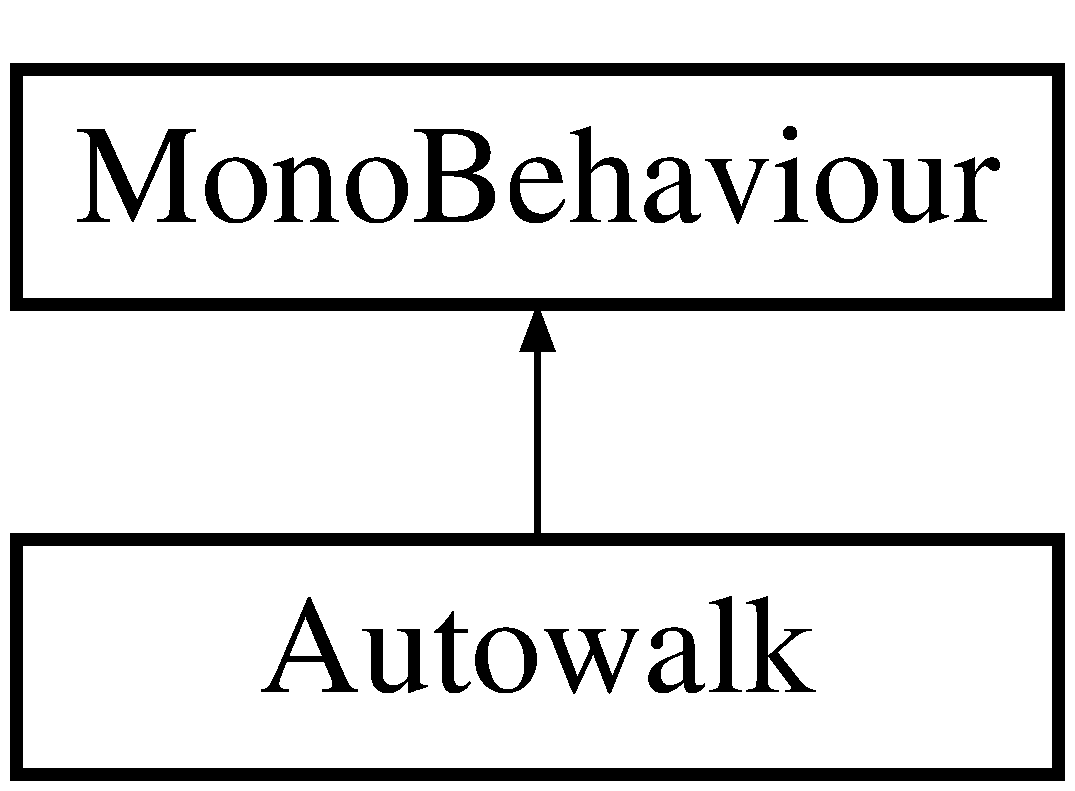
\includegraphics[height=2.000000cm]{class_autowalk}
\end{center}
\end{figure}
\subsection*{Public Attributes}
\begin{DoxyCompactItemize}
\item 
float \hyperlink{class_autowalk_a3092a4d8988a54c5774865800cef6c22}{speed}
\item 
bool \hyperlink{class_autowalk_ac644a9b75f6f5ace1155fd461ba7afc5}{walk\+When\+Triggered}
\item 
bool \hyperlink{class_autowalk_aa93343a7a4e1f3884c91cbbe7cdfea1f}{walk\+When\+Look\+Down}
\item 
bool \hyperlink{class_autowalk_afb9baa3b1db7ced136fc83fca8a40f9a}{freeze\+Y\+Position}
\item 
float \hyperlink{class_autowalk_a65b75b93ffed0edfd3fdf00b2f03fcc6}{y\+Offset}
\item 
double \hyperlink{class_autowalk_a88a1c42da0a6619e6f5540b1ff823e2a}{threshold\+Angle}
\end{DoxyCompactItemize}


\subsection{Member Data Documentation}
\hypertarget{class_autowalk_afb9baa3b1db7ced136fc83fca8a40f9a}{}\index{Autowalk@{Autowalk}!freeze\+Y\+Position@{freeze\+Y\+Position}}
\index{freeze\+Y\+Position@{freeze\+Y\+Position}!Autowalk@{Autowalk}}
\subsubsection[{freeze\+Y\+Position}]{\setlength{\rightskip}{0pt plus 5cm}bool Autowalk.\+freeze\+Y\+Position}\label{class_autowalk_afb9baa3b1db7ced136fc83fca8a40f9a}
\hypertarget{class_autowalk_a3092a4d8988a54c5774865800cef6c22}{}\index{Autowalk@{Autowalk}!speed@{speed}}
\index{speed@{speed}!Autowalk@{Autowalk}}
\subsubsection[{speed}]{\setlength{\rightskip}{0pt plus 5cm}float Autowalk.\+speed}\label{class_autowalk_a3092a4d8988a54c5774865800cef6c22}
\hypertarget{class_autowalk_a88a1c42da0a6619e6f5540b1ff823e2a}{}\index{Autowalk@{Autowalk}!threshold\+Angle@{threshold\+Angle}}
\index{threshold\+Angle@{threshold\+Angle}!Autowalk@{Autowalk}}
\subsubsection[{threshold\+Angle}]{\setlength{\rightskip}{0pt plus 5cm}double Autowalk.\+threshold\+Angle}\label{class_autowalk_a88a1c42da0a6619e6f5540b1ff823e2a}
\hypertarget{class_autowalk_aa93343a7a4e1f3884c91cbbe7cdfea1f}{}\index{Autowalk@{Autowalk}!walk\+When\+Look\+Down@{walk\+When\+Look\+Down}}
\index{walk\+When\+Look\+Down@{walk\+When\+Look\+Down}!Autowalk@{Autowalk}}
\subsubsection[{walk\+When\+Look\+Down}]{\setlength{\rightskip}{0pt plus 5cm}bool Autowalk.\+walk\+When\+Look\+Down}\label{class_autowalk_aa93343a7a4e1f3884c91cbbe7cdfea1f}
\hypertarget{class_autowalk_ac644a9b75f6f5ace1155fd461ba7afc5}{}\index{Autowalk@{Autowalk}!walk\+When\+Triggered@{walk\+When\+Triggered}}
\index{walk\+When\+Triggered@{walk\+When\+Triggered}!Autowalk@{Autowalk}}
\subsubsection[{walk\+When\+Triggered}]{\setlength{\rightskip}{0pt plus 5cm}bool Autowalk.\+walk\+When\+Triggered}\label{class_autowalk_ac644a9b75f6f5ace1155fd461ba7afc5}
\hypertarget{class_autowalk_a65b75b93ffed0edfd3fdf00b2f03fcc6}{}\index{Autowalk@{Autowalk}!y\+Offset@{y\+Offset}}
\index{y\+Offset@{y\+Offset}!Autowalk@{Autowalk}}
\subsubsection[{y\+Offset}]{\setlength{\rightskip}{0pt plus 5cm}float Autowalk.\+y\+Offset}\label{class_autowalk_a65b75b93ffed0edfd3fdf00b2f03fcc6}


The documentation for this class was generated from the following file\+:\begin{DoxyCompactItemize}
\item 
\hyperlink{_autowalk_8cs}{Autowalk.\+cs}\end{DoxyCompactItemize}

\hypertarget{class_character_motor}{}\section{Character\+Motor Class Reference}
\label{class_character_motor}\index{Character\+Motor@{Character\+Motor}}
Inheritance diagram for Character\+Motor\+:\begin{figure}[H]
\begin{center}
\leavevmode
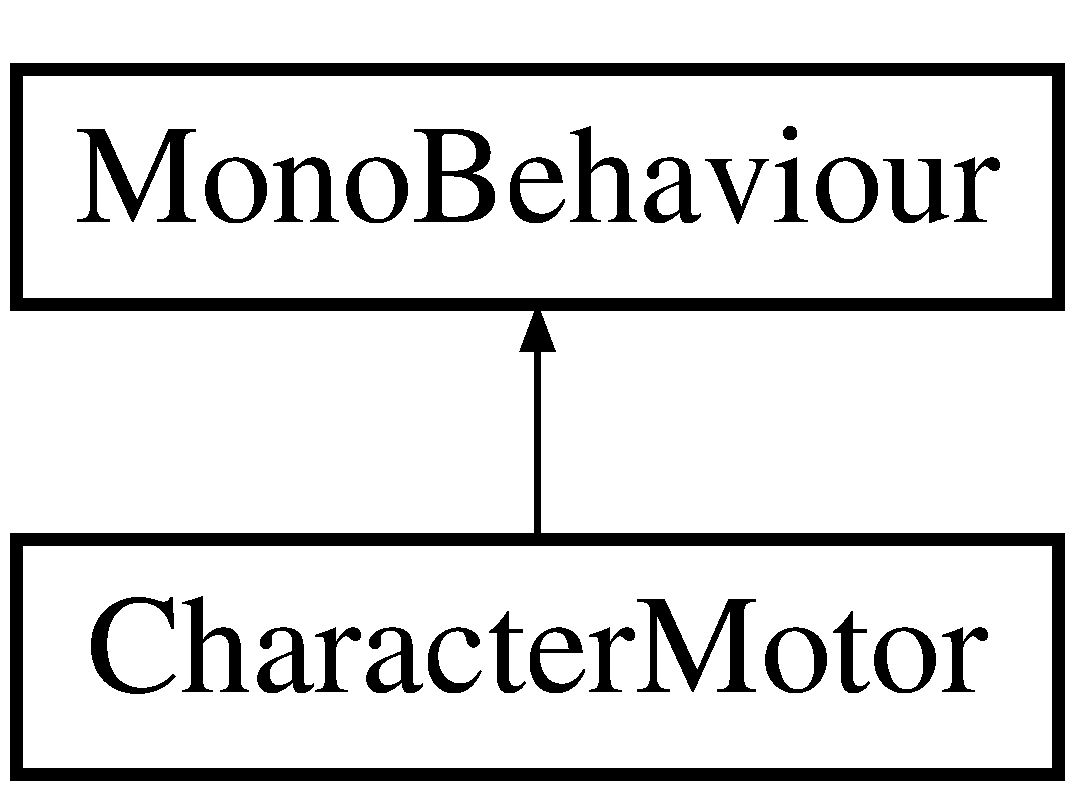
\includegraphics[height=2.000000cm]{class_character_motor}
\end{center}
\end{figure}
\subsection*{Classes}
\begin{DoxyCompactItemize}
\item 
class \hyperlink{class_character_motor_1_1_character_motor_jumping}{Character\+Motor\+Jumping}
\item 
class \hyperlink{class_character_motor_1_1_character_motor_movement}{Character\+Motor\+Movement}
\item 
class \hyperlink{class_character_motor_1_1_character_motor_moving_platform}{Character\+Motor\+Moving\+Platform}
\item 
class \hyperlink{class_character_motor_1_1_character_motor_sliding}{Character\+Motor\+Sliding}
\end{DoxyCompactItemize}
\subsection*{Public Types}
\begin{DoxyCompactItemize}
\item 
enum \hyperlink{class_character_motor_ae8904b1ae7907502123f9376cf77a045}{Movement\+Transfer\+On\+Jump} \{ \hyperlink{class_character_motor_ae8904b1ae7907502123f9376cf77a045a6adf97f83acf6453d4a6a4b1070f3754}{Movement\+Transfer\+On\+Jump.\+None}, 
\hyperlink{class_character_motor_ae8904b1ae7907502123f9376cf77a045a58ffcf57c2b00a9e42d67e43391ca652}{Movement\+Transfer\+On\+Jump.\+Init\+Transfer}, 
\hyperlink{class_character_motor_ae8904b1ae7907502123f9376cf77a045a1caa5cdb42cd1fe12e5047b8aaa499b9}{Movement\+Transfer\+On\+Jump.\+Perma\+Transfer}, 
\hyperlink{class_character_motor_ae8904b1ae7907502123f9376cf77a045af922013cd8da7d5623b13b9b520bacc3}{Movement\+Transfer\+On\+Jump.\+Perma\+Locked}
 \}
\end{DoxyCompactItemize}
\subsection*{Public Attributes}
\begin{DoxyCompactItemize}
\item 
Vector3 \hyperlink{class_character_motor_ad0bcb8698b03c87100f137eda3d44778}{input\+Move\+Direction} = Vector3.\+zero
\item 
bool \hyperlink{class_character_motor_a35e7c3109338c4d66e8a0e3e8267eb1c}{input\+Jump} = false
\item 
\hyperlink{class_character_motor_1_1_character_motor_movement}{Character\+Motor\+Movement} \hyperlink{class_character_motor_a4e78119cee0a5fefef9e00fa3e3226e6}{movement} = new \hyperlink{class_character_motor_1_1_character_motor_movement}{Character\+Motor\+Movement}()
\item 
\hyperlink{class_character_motor_1_1_character_motor_jumping}{Character\+Motor\+Jumping} \hyperlink{class_character_motor_ae37632c27e5831d2abebfaf6f3f1090d}{jumping} = new \hyperlink{class_character_motor_1_1_character_motor_jumping}{Character\+Motor\+Jumping}()
\item 
\hyperlink{class_character_motor_1_1_character_motor_moving_platform}{Character\+Motor\+Moving\+Platform} \hyperlink{class_character_motor_a7e1365cba58a6219df462088ee282bbb}{moving\+Platform} = new \hyperlink{class_character_motor_1_1_character_motor_moving_platform}{Character\+Motor\+Moving\+Platform}()
\item 
\hyperlink{class_character_motor_1_1_character_motor_sliding}{Character\+Motor\+Sliding} \hyperlink{class_character_motor_acdffbadbd84cdc50a57ae1675166ceb5}{sliding} = new \hyperlink{class_character_motor_1_1_character_motor_sliding}{Character\+Motor\+Sliding}()
\item 
bool \hyperlink{class_character_motor_a2515921b1c3156e2a4a15a7faf13a222}{grounded} = true
\item 
Vector3 \hyperlink{class_character_motor_a83cfb98714aa374ddef3692ccd8cba2c}{ground\+Normal} = Vector3.\+zero
\end{DoxyCompactItemize}


\subsection{Member Enumeration Documentation}
\hypertarget{class_character_motor_ae8904b1ae7907502123f9376cf77a045}{}\index{Character\+Motor@{Character\+Motor}!Movement\+Transfer\+On\+Jump@{Movement\+Transfer\+On\+Jump}}
\index{Movement\+Transfer\+On\+Jump@{Movement\+Transfer\+On\+Jump}!Character\+Motor@{Character\+Motor}}
\subsubsection[{Movement\+Transfer\+On\+Jump}]{\setlength{\rightskip}{0pt plus 5cm}enum {\bf Character\+Motor.\+Movement\+Transfer\+On\+Jump}\hspace{0.3cm}{\ttfamily [strong]}}\label{class_character_motor_ae8904b1ae7907502123f9376cf77a045}
\begin{Desc}
\item[Enumerator]\par
\begin{description}
\index{None@{None}!Character\+Motor@{Character\+Motor}}\index{Character\+Motor@{Character\+Motor}!None@{None}}\item[{\em 
\hypertarget{class_character_motor_ae8904b1ae7907502123f9376cf77a045a6adf97f83acf6453d4a6a4b1070f3754}{}None\label{class_character_motor_ae8904b1ae7907502123f9376cf77a045a6adf97f83acf6453d4a6a4b1070f3754}
}]\index{Init\+Transfer@{Init\+Transfer}!Character\+Motor@{Character\+Motor}}\index{Character\+Motor@{Character\+Motor}!Init\+Transfer@{Init\+Transfer}}\item[{\em 
\hypertarget{class_character_motor_ae8904b1ae7907502123f9376cf77a045a58ffcf57c2b00a9e42d67e43391ca652}{}Init\+Transfer\label{class_character_motor_ae8904b1ae7907502123f9376cf77a045a58ffcf57c2b00a9e42d67e43391ca652}
}]\index{Perma\+Transfer@{Perma\+Transfer}!Character\+Motor@{Character\+Motor}}\index{Character\+Motor@{Character\+Motor}!Perma\+Transfer@{Perma\+Transfer}}\item[{\em 
\hypertarget{class_character_motor_ae8904b1ae7907502123f9376cf77a045a1caa5cdb42cd1fe12e5047b8aaa499b9}{}Perma\+Transfer\label{class_character_motor_ae8904b1ae7907502123f9376cf77a045a1caa5cdb42cd1fe12e5047b8aaa499b9}
}]\index{Perma\+Locked@{Perma\+Locked}!Character\+Motor@{Character\+Motor}}\index{Character\+Motor@{Character\+Motor}!Perma\+Locked@{Perma\+Locked}}\item[{\em 
\hypertarget{class_character_motor_ae8904b1ae7907502123f9376cf77a045af922013cd8da7d5623b13b9b520bacc3}{}Perma\+Locked\label{class_character_motor_ae8904b1ae7907502123f9376cf77a045af922013cd8da7d5623b13b9b520bacc3}
}]\end{description}
\end{Desc}


\subsection{Member Data Documentation}
\hypertarget{class_character_motor_a2515921b1c3156e2a4a15a7faf13a222}{}\index{Character\+Motor@{Character\+Motor}!grounded@{grounded}}
\index{grounded@{grounded}!Character\+Motor@{Character\+Motor}}
\subsubsection[{grounded}]{\setlength{\rightskip}{0pt plus 5cm}bool Character\+Motor.\+grounded = true}\label{class_character_motor_a2515921b1c3156e2a4a15a7faf13a222}
\hypertarget{class_character_motor_a83cfb98714aa374ddef3692ccd8cba2c}{}\index{Character\+Motor@{Character\+Motor}!ground\+Normal@{ground\+Normal}}
\index{ground\+Normal@{ground\+Normal}!Character\+Motor@{Character\+Motor}}
\subsubsection[{ground\+Normal}]{\setlength{\rightskip}{0pt plus 5cm}Vector3 Character\+Motor.\+ground\+Normal = Vector3.\+zero}\label{class_character_motor_a83cfb98714aa374ddef3692ccd8cba2c}
\hypertarget{class_character_motor_a35e7c3109338c4d66e8a0e3e8267eb1c}{}\index{Character\+Motor@{Character\+Motor}!input\+Jump@{input\+Jump}}
\index{input\+Jump@{input\+Jump}!Character\+Motor@{Character\+Motor}}
\subsubsection[{input\+Jump}]{\setlength{\rightskip}{0pt plus 5cm}bool Character\+Motor.\+input\+Jump = false}\label{class_character_motor_a35e7c3109338c4d66e8a0e3e8267eb1c}
\hypertarget{class_character_motor_ad0bcb8698b03c87100f137eda3d44778}{}\index{Character\+Motor@{Character\+Motor}!input\+Move\+Direction@{input\+Move\+Direction}}
\index{input\+Move\+Direction@{input\+Move\+Direction}!Character\+Motor@{Character\+Motor}}
\subsubsection[{input\+Move\+Direction}]{\setlength{\rightskip}{0pt plus 5cm}Vector3 Character\+Motor.\+input\+Move\+Direction = Vector3.\+zero}\label{class_character_motor_ad0bcb8698b03c87100f137eda3d44778}
\hypertarget{class_character_motor_ae37632c27e5831d2abebfaf6f3f1090d}{}\index{Character\+Motor@{Character\+Motor}!jumping@{jumping}}
\index{jumping@{jumping}!Character\+Motor@{Character\+Motor}}
\subsubsection[{jumping}]{\setlength{\rightskip}{0pt plus 5cm}{\bf Character\+Motor\+Jumping} Character\+Motor.\+jumping = new {\bf Character\+Motor\+Jumping}()}\label{class_character_motor_ae37632c27e5831d2abebfaf6f3f1090d}
\hypertarget{class_character_motor_a4e78119cee0a5fefef9e00fa3e3226e6}{}\index{Character\+Motor@{Character\+Motor}!movement@{movement}}
\index{movement@{movement}!Character\+Motor@{Character\+Motor}}
\subsubsection[{movement}]{\setlength{\rightskip}{0pt plus 5cm}{\bf Character\+Motor\+Movement} Character\+Motor.\+movement = new {\bf Character\+Motor\+Movement}()}\label{class_character_motor_a4e78119cee0a5fefef9e00fa3e3226e6}
\hypertarget{class_character_motor_a7e1365cba58a6219df462088ee282bbb}{}\index{Character\+Motor@{Character\+Motor}!moving\+Platform@{moving\+Platform}}
\index{moving\+Platform@{moving\+Platform}!Character\+Motor@{Character\+Motor}}
\subsubsection[{moving\+Platform}]{\setlength{\rightskip}{0pt plus 5cm}{\bf Character\+Motor\+Moving\+Platform} Character\+Motor.\+moving\+Platform = new {\bf Character\+Motor\+Moving\+Platform}()}\label{class_character_motor_a7e1365cba58a6219df462088ee282bbb}
\hypertarget{class_character_motor_acdffbadbd84cdc50a57ae1675166ceb5}{}\index{Character\+Motor@{Character\+Motor}!sliding@{sliding}}
\index{sliding@{sliding}!Character\+Motor@{Character\+Motor}}
\subsubsection[{sliding}]{\setlength{\rightskip}{0pt plus 5cm}{\bf Character\+Motor\+Sliding} Character\+Motor.\+sliding = new {\bf Character\+Motor\+Sliding}()}\label{class_character_motor_acdffbadbd84cdc50a57ae1675166ceb5}


The documentation for this class was generated from the following file\+:\begin{DoxyCompactItemize}
\item 
\hyperlink{_character_motor_8cs}{Character\+Motor.\+cs}\end{DoxyCompactItemize}

\hypertarget{class_character_motor_1_1_character_motor_jumping}{}\section{Character\+Motor.\+Character\+Motor\+Jumping Class Reference}
\label{class_character_motor_1_1_character_motor_jumping}\index{Character\+Motor.\+Character\+Motor\+Jumping@{Character\+Motor.\+Character\+Motor\+Jumping}}
\subsection*{Public Attributes}
\begin{DoxyCompactItemize}
\item 
bool \hyperlink{class_character_motor_1_1_character_motor_jumping_af23d1cf82e83080be778b7566655c6bd}{enabled} = true
\item 
float \hyperlink{class_character_motor_1_1_character_motor_jumping_acf5b43f27a4f1c30950c9854910af59f}{base\+Height} = 1.\+0f
\item 
float \hyperlink{class_character_motor_1_1_character_motor_jumping_a40c3590760b261e0dd8e11538dd1bd9f}{extra\+Height} = 4.\+1f
\item 
float \hyperlink{class_character_motor_1_1_character_motor_jumping_ae234d27fc10de24027da0f635f076d9f}{perp\+Amount} = 0.\+0f
\item 
float \hyperlink{class_character_motor_1_1_character_motor_jumping_a555ce2e43e9c5f121139647afe909f81}{steep\+Perp\+Amount} = 0.\+5f
\item 
bool \hyperlink{class_character_motor_1_1_character_motor_jumping_a99a2b72de5db18d6bb8d38ae6128fdf0}{jumping} = false
\item 
bool \hyperlink{class_character_motor_1_1_character_motor_jumping_aea7df563698079085372631e65b52931}{holding\+Jump\+Button} = false
\item 
float \hyperlink{class_character_motor_1_1_character_motor_jumping_a15c702232012b6d8bf59a21ecbd63455}{last\+Start\+Time} = 0.\+0f
\item 
float \hyperlink{class_character_motor_1_1_character_motor_jumping_a99ec2b16436dd52fc944eb44af8c2758}{last\+Button\+Down\+Time} = -\/100.\+0f
\item 
Vector3 \hyperlink{class_character_motor_1_1_character_motor_jumping_ac3a3c23224ab13d585a7860231ed9dd9}{jump\+Dir} = Vector3.\+up
\end{DoxyCompactItemize}


\subsection{Member Data Documentation}
\hypertarget{class_character_motor_1_1_character_motor_jumping_acf5b43f27a4f1c30950c9854910af59f}{}\index{Character\+Motor\+::\+Character\+Motor\+Jumping@{Character\+Motor\+::\+Character\+Motor\+Jumping}!base\+Height@{base\+Height}}
\index{base\+Height@{base\+Height}!Character\+Motor\+::\+Character\+Motor\+Jumping@{Character\+Motor\+::\+Character\+Motor\+Jumping}}
\subsubsection[{base\+Height}]{\setlength{\rightskip}{0pt plus 5cm}float Character\+Motor.\+Character\+Motor\+Jumping.\+base\+Height = 1.\+0f}\label{class_character_motor_1_1_character_motor_jumping_acf5b43f27a4f1c30950c9854910af59f}
\hypertarget{class_character_motor_1_1_character_motor_jumping_af23d1cf82e83080be778b7566655c6bd}{}\index{Character\+Motor\+::\+Character\+Motor\+Jumping@{Character\+Motor\+::\+Character\+Motor\+Jumping}!enabled@{enabled}}
\index{enabled@{enabled}!Character\+Motor\+::\+Character\+Motor\+Jumping@{Character\+Motor\+::\+Character\+Motor\+Jumping}}
\subsubsection[{enabled}]{\setlength{\rightskip}{0pt plus 5cm}bool Character\+Motor.\+Character\+Motor\+Jumping.\+enabled = true}\label{class_character_motor_1_1_character_motor_jumping_af23d1cf82e83080be778b7566655c6bd}
\hypertarget{class_character_motor_1_1_character_motor_jumping_a40c3590760b261e0dd8e11538dd1bd9f}{}\index{Character\+Motor\+::\+Character\+Motor\+Jumping@{Character\+Motor\+::\+Character\+Motor\+Jumping}!extra\+Height@{extra\+Height}}
\index{extra\+Height@{extra\+Height}!Character\+Motor\+::\+Character\+Motor\+Jumping@{Character\+Motor\+::\+Character\+Motor\+Jumping}}
\subsubsection[{extra\+Height}]{\setlength{\rightskip}{0pt plus 5cm}float Character\+Motor.\+Character\+Motor\+Jumping.\+extra\+Height = 4.\+1f}\label{class_character_motor_1_1_character_motor_jumping_a40c3590760b261e0dd8e11538dd1bd9f}
\hypertarget{class_character_motor_1_1_character_motor_jumping_aea7df563698079085372631e65b52931}{}\index{Character\+Motor\+::\+Character\+Motor\+Jumping@{Character\+Motor\+::\+Character\+Motor\+Jumping}!holding\+Jump\+Button@{holding\+Jump\+Button}}
\index{holding\+Jump\+Button@{holding\+Jump\+Button}!Character\+Motor\+::\+Character\+Motor\+Jumping@{Character\+Motor\+::\+Character\+Motor\+Jumping}}
\subsubsection[{holding\+Jump\+Button}]{\setlength{\rightskip}{0pt plus 5cm}bool Character\+Motor.\+Character\+Motor\+Jumping.\+holding\+Jump\+Button = false}\label{class_character_motor_1_1_character_motor_jumping_aea7df563698079085372631e65b52931}
\hypertarget{class_character_motor_1_1_character_motor_jumping_ac3a3c23224ab13d585a7860231ed9dd9}{}\index{Character\+Motor\+::\+Character\+Motor\+Jumping@{Character\+Motor\+::\+Character\+Motor\+Jumping}!jump\+Dir@{jump\+Dir}}
\index{jump\+Dir@{jump\+Dir}!Character\+Motor\+::\+Character\+Motor\+Jumping@{Character\+Motor\+::\+Character\+Motor\+Jumping}}
\subsubsection[{jump\+Dir}]{\setlength{\rightskip}{0pt plus 5cm}Vector3 Character\+Motor.\+Character\+Motor\+Jumping.\+jump\+Dir = Vector3.\+up}\label{class_character_motor_1_1_character_motor_jumping_ac3a3c23224ab13d585a7860231ed9dd9}
\hypertarget{class_character_motor_1_1_character_motor_jumping_a99a2b72de5db18d6bb8d38ae6128fdf0}{}\index{Character\+Motor\+::\+Character\+Motor\+Jumping@{Character\+Motor\+::\+Character\+Motor\+Jumping}!jumping@{jumping}}
\index{jumping@{jumping}!Character\+Motor\+::\+Character\+Motor\+Jumping@{Character\+Motor\+::\+Character\+Motor\+Jumping}}
\subsubsection[{jumping}]{\setlength{\rightskip}{0pt plus 5cm}bool Character\+Motor.\+Character\+Motor\+Jumping.\+jumping = false}\label{class_character_motor_1_1_character_motor_jumping_a99a2b72de5db18d6bb8d38ae6128fdf0}
\hypertarget{class_character_motor_1_1_character_motor_jumping_a99ec2b16436dd52fc944eb44af8c2758}{}\index{Character\+Motor\+::\+Character\+Motor\+Jumping@{Character\+Motor\+::\+Character\+Motor\+Jumping}!last\+Button\+Down\+Time@{last\+Button\+Down\+Time}}
\index{last\+Button\+Down\+Time@{last\+Button\+Down\+Time}!Character\+Motor\+::\+Character\+Motor\+Jumping@{Character\+Motor\+::\+Character\+Motor\+Jumping}}
\subsubsection[{last\+Button\+Down\+Time}]{\setlength{\rightskip}{0pt plus 5cm}float Character\+Motor.\+Character\+Motor\+Jumping.\+last\+Button\+Down\+Time = -\/100.\+0f}\label{class_character_motor_1_1_character_motor_jumping_a99ec2b16436dd52fc944eb44af8c2758}
\hypertarget{class_character_motor_1_1_character_motor_jumping_a15c702232012b6d8bf59a21ecbd63455}{}\index{Character\+Motor\+::\+Character\+Motor\+Jumping@{Character\+Motor\+::\+Character\+Motor\+Jumping}!last\+Start\+Time@{last\+Start\+Time}}
\index{last\+Start\+Time@{last\+Start\+Time}!Character\+Motor\+::\+Character\+Motor\+Jumping@{Character\+Motor\+::\+Character\+Motor\+Jumping}}
\subsubsection[{last\+Start\+Time}]{\setlength{\rightskip}{0pt plus 5cm}float Character\+Motor.\+Character\+Motor\+Jumping.\+last\+Start\+Time = 0.\+0f}\label{class_character_motor_1_1_character_motor_jumping_a15c702232012b6d8bf59a21ecbd63455}
\hypertarget{class_character_motor_1_1_character_motor_jumping_ae234d27fc10de24027da0f635f076d9f}{}\index{Character\+Motor\+::\+Character\+Motor\+Jumping@{Character\+Motor\+::\+Character\+Motor\+Jumping}!perp\+Amount@{perp\+Amount}}
\index{perp\+Amount@{perp\+Amount}!Character\+Motor\+::\+Character\+Motor\+Jumping@{Character\+Motor\+::\+Character\+Motor\+Jumping}}
\subsubsection[{perp\+Amount}]{\setlength{\rightskip}{0pt plus 5cm}float Character\+Motor.\+Character\+Motor\+Jumping.\+perp\+Amount = 0.\+0f}\label{class_character_motor_1_1_character_motor_jumping_ae234d27fc10de24027da0f635f076d9f}
\hypertarget{class_character_motor_1_1_character_motor_jumping_a555ce2e43e9c5f121139647afe909f81}{}\index{Character\+Motor\+::\+Character\+Motor\+Jumping@{Character\+Motor\+::\+Character\+Motor\+Jumping}!steep\+Perp\+Amount@{steep\+Perp\+Amount}}
\index{steep\+Perp\+Amount@{steep\+Perp\+Amount}!Character\+Motor\+::\+Character\+Motor\+Jumping@{Character\+Motor\+::\+Character\+Motor\+Jumping}}
\subsubsection[{steep\+Perp\+Amount}]{\setlength{\rightskip}{0pt plus 5cm}float Character\+Motor.\+Character\+Motor\+Jumping.\+steep\+Perp\+Amount = 0.\+5f}\label{class_character_motor_1_1_character_motor_jumping_a555ce2e43e9c5f121139647afe909f81}


The documentation for this class was generated from the following file\+:\begin{DoxyCompactItemize}
\item 
\hyperlink{_character_motor_8cs}{Character\+Motor.\+cs}\end{DoxyCompactItemize}

\hypertarget{class_character_motor_1_1_character_motor_movement}{}\section{Character\+Motor.\+Character\+Motor\+Movement Class Reference}
\label{class_character_motor_1_1_character_motor_movement}\index{Character\+Motor.\+Character\+Motor\+Movement@{Character\+Motor.\+Character\+Motor\+Movement}}
\subsection*{Public Attributes}
\begin{DoxyCompactItemize}
\item 
float \hyperlink{class_character_motor_1_1_character_motor_movement_aa820360350daf9692ded079eb05a9556}{max\+Forward\+Speed} = 3.\+0f
\item 
float \hyperlink{class_character_motor_1_1_character_motor_movement_a027288f30c506ef80b64ea0903642d03}{max\+Sideways\+Speed} = 2.\+0f
\item 
float \hyperlink{class_character_motor_1_1_character_motor_movement_a2f6ed24c7e60a10e62aefa33741b0eb5}{max\+Backwards\+Speed} = 2.\+0f
\item 
Animation\+Curve \hyperlink{class_character_motor_1_1_character_motor_movement_ab157f4037ba87d83810d2bf59b78803e}{slope\+Speed\+Multiplier} = new Animation\+Curve(new Keyframe(-\/90, 1), new Keyframe(0, 1), new Keyframe(90, 0))
\item 
float \hyperlink{class_character_motor_1_1_character_motor_movement_a0968f793fea8120298e5ec2d721ec3a2}{max\+Ground\+Acceleration} = 30.\+0f
\item 
float \hyperlink{class_character_motor_1_1_character_motor_movement_a0a985e4edd7576f3657d379972dc077e}{max\+Air\+Acceleration} = 20.\+0f
\item 
float \hyperlink{class_character_motor_1_1_character_motor_movement_ac8c8626de028fa14bd370baef3ac4393}{gravity} = 9.\+81f
\item 
float \hyperlink{class_character_motor_1_1_character_motor_movement_ae41d6a91868b3664fe183b45bf831505}{max\+Fall\+Speed} = 20.\+0f
\item 
Collision\+Flags \hyperlink{class_character_motor_1_1_character_motor_movement_aac4344120b66bff82cbfb55b388cde77}{collision\+Flags}
\item 
Vector3 \hyperlink{class_character_motor_1_1_character_motor_movement_a602814fda948d4dbc79a2b4f18386ce1}{velocity}
\item 
Vector3 \hyperlink{class_character_motor_1_1_character_motor_movement_a9a11d4502ed9cb50922c1198093af7b3}{frame\+Velocity} = Vector3.\+zero
\item 
Vector3 \hyperlink{class_character_motor_1_1_character_motor_movement_a359dedb4d215a06ebc2b81a137634d4a}{hit\+Point} = Vector3.\+zero
\item 
Vector3 \hyperlink{class_character_motor_1_1_character_motor_movement_a10fee81a506f0445be8905e3de83a0bc}{last\+Hit\+Point} = new Vector3(Mathf.\+Infinity, 0, 0)
\end{DoxyCompactItemize}


\subsection{Member Data Documentation}
\hypertarget{class_character_motor_1_1_character_motor_movement_aac4344120b66bff82cbfb55b388cde77}{}\index{Character\+Motor\+::\+Character\+Motor\+Movement@{Character\+Motor\+::\+Character\+Motor\+Movement}!collision\+Flags@{collision\+Flags}}
\index{collision\+Flags@{collision\+Flags}!Character\+Motor\+::\+Character\+Motor\+Movement@{Character\+Motor\+::\+Character\+Motor\+Movement}}
\subsubsection[{collision\+Flags}]{\setlength{\rightskip}{0pt plus 5cm}Collision\+Flags Character\+Motor.\+Character\+Motor\+Movement.\+collision\+Flags}\label{class_character_motor_1_1_character_motor_movement_aac4344120b66bff82cbfb55b388cde77}
\hypertarget{class_character_motor_1_1_character_motor_movement_a9a11d4502ed9cb50922c1198093af7b3}{}\index{Character\+Motor\+::\+Character\+Motor\+Movement@{Character\+Motor\+::\+Character\+Motor\+Movement}!frame\+Velocity@{frame\+Velocity}}
\index{frame\+Velocity@{frame\+Velocity}!Character\+Motor\+::\+Character\+Motor\+Movement@{Character\+Motor\+::\+Character\+Motor\+Movement}}
\subsubsection[{frame\+Velocity}]{\setlength{\rightskip}{0pt plus 5cm}Vector3 Character\+Motor.\+Character\+Motor\+Movement.\+frame\+Velocity = Vector3.\+zero}\label{class_character_motor_1_1_character_motor_movement_a9a11d4502ed9cb50922c1198093af7b3}
\hypertarget{class_character_motor_1_1_character_motor_movement_ac8c8626de028fa14bd370baef3ac4393}{}\index{Character\+Motor\+::\+Character\+Motor\+Movement@{Character\+Motor\+::\+Character\+Motor\+Movement}!gravity@{gravity}}
\index{gravity@{gravity}!Character\+Motor\+::\+Character\+Motor\+Movement@{Character\+Motor\+::\+Character\+Motor\+Movement}}
\subsubsection[{gravity}]{\setlength{\rightskip}{0pt plus 5cm}float Character\+Motor.\+Character\+Motor\+Movement.\+gravity = 9.\+81f}\label{class_character_motor_1_1_character_motor_movement_ac8c8626de028fa14bd370baef3ac4393}
\hypertarget{class_character_motor_1_1_character_motor_movement_a359dedb4d215a06ebc2b81a137634d4a}{}\index{Character\+Motor\+::\+Character\+Motor\+Movement@{Character\+Motor\+::\+Character\+Motor\+Movement}!hit\+Point@{hit\+Point}}
\index{hit\+Point@{hit\+Point}!Character\+Motor\+::\+Character\+Motor\+Movement@{Character\+Motor\+::\+Character\+Motor\+Movement}}
\subsubsection[{hit\+Point}]{\setlength{\rightskip}{0pt plus 5cm}Vector3 Character\+Motor.\+Character\+Motor\+Movement.\+hit\+Point = Vector3.\+zero}\label{class_character_motor_1_1_character_motor_movement_a359dedb4d215a06ebc2b81a137634d4a}
\hypertarget{class_character_motor_1_1_character_motor_movement_a10fee81a506f0445be8905e3de83a0bc}{}\index{Character\+Motor\+::\+Character\+Motor\+Movement@{Character\+Motor\+::\+Character\+Motor\+Movement}!last\+Hit\+Point@{last\+Hit\+Point}}
\index{last\+Hit\+Point@{last\+Hit\+Point}!Character\+Motor\+::\+Character\+Motor\+Movement@{Character\+Motor\+::\+Character\+Motor\+Movement}}
\subsubsection[{last\+Hit\+Point}]{\setlength{\rightskip}{0pt plus 5cm}Vector3 Character\+Motor.\+Character\+Motor\+Movement.\+last\+Hit\+Point = new Vector3(Mathf.\+Infinity, 0, 0)}\label{class_character_motor_1_1_character_motor_movement_a10fee81a506f0445be8905e3de83a0bc}
\hypertarget{class_character_motor_1_1_character_motor_movement_a0a985e4edd7576f3657d379972dc077e}{}\index{Character\+Motor\+::\+Character\+Motor\+Movement@{Character\+Motor\+::\+Character\+Motor\+Movement}!max\+Air\+Acceleration@{max\+Air\+Acceleration}}
\index{max\+Air\+Acceleration@{max\+Air\+Acceleration}!Character\+Motor\+::\+Character\+Motor\+Movement@{Character\+Motor\+::\+Character\+Motor\+Movement}}
\subsubsection[{max\+Air\+Acceleration}]{\setlength{\rightskip}{0pt plus 5cm}float Character\+Motor.\+Character\+Motor\+Movement.\+max\+Air\+Acceleration = 20.\+0f}\label{class_character_motor_1_1_character_motor_movement_a0a985e4edd7576f3657d379972dc077e}
\hypertarget{class_character_motor_1_1_character_motor_movement_a2f6ed24c7e60a10e62aefa33741b0eb5}{}\index{Character\+Motor\+::\+Character\+Motor\+Movement@{Character\+Motor\+::\+Character\+Motor\+Movement}!max\+Backwards\+Speed@{max\+Backwards\+Speed}}
\index{max\+Backwards\+Speed@{max\+Backwards\+Speed}!Character\+Motor\+::\+Character\+Motor\+Movement@{Character\+Motor\+::\+Character\+Motor\+Movement}}
\subsubsection[{max\+Backwards\+Speed}]{\setlength{\rightskip}{0pt plus 5cm}float Character\+Motor.\+Character\+Motor\+Movement.\+max\+Backwards\+Speed = 2.\+0f}\label{class_character_motor_1_1_character_motor_movement_a2f6ed24c7e60a10e62aefa33741b0eb5}
\hypertarget{class_character_motor_1_1_character_motor_movement_ae41d6a91868b3664fe183b45bf831505}{}\index{Character\+Motor\+::\+Character\+Motor\+Movement@{Character\+Motor\+::\+Character\+Motor\+Movement}!max\+Fall\+Speed@{max\+Fall\+Speed}}
\index{max\+Fall\+Speed@{max\+Fall\+Speed}!Character\+Motor\+::\+Character\+Motor\+Movement@{Character\+Motor\+::\+Character\+Motor\+Movement}}
\subsubsection[{max\+Fall\+Speed}]{\setlength{\rightskip}{0pt plus 5cm}float Character\+Motor.\+Character\+Motor\+Movement.\+max\+Fall\+Speed = 20.\+0f}\label{class_character_motor_1_1_character_motor_movement_ae41d6a91868b3664fe183b45bf831505}
\hypertarget{class_character_motor_1_1_character_motor_movement_aa820360350daf9692ded079eb05a9556}{}\index{Character\+Motor\+::\+Character\+Motor\+Movement@{Character\+Motor\+::\+Character\+Motor\+Movement}!max\+Forward\+Speed@{max\+Forward\+Speed}}
\index{max\+Forward\+Speed@{max\+Forward\+Speed}!Character\+Motor\+::\+Character\+Motor\+Movement@{Character\+Motor\+::\+Character\+Motor\+Movement}}
\subsubsection[{max\+Forward\+Speed}]{\setlength{\rightskip}{0pt plus 5cm}float Character\+Motor.\+Character\+Motor\+Movement.\+max\+Forward\+Speed = 3.\+0f}\label{class_character_motor_1_1_character_motor_movement_aa820360350daf9692ded079eb05a9556}
\hypertarget{class_character_motor_1_1_character_motor_movement_a0968f793fea8120298e5ec2d721ec3a2}{}\index{Character\+Motor\+::\+Character\+Motor\+Movement@{Character\+Motor\+::\+Character\+Motor\+Movement}!max\+Ground\+Acceleration@{max\+Ground\+Acceleration}}
\index{max\+Ground\+Acceleration@{max\+Ground\+Acceleration}!Character\+Motor\+::\+Character\+Motor\+Movement@{Character\+Motor\+::\+Character\+Motor\+Movement}}
\subsubsection[{max\+Ground\+Acceleration}]{\setlength{\rightskip}{0pt plus 5cm}float Character\+Motor.\+Character\+Motor\+Movement.\+max\+Ground\+Acceleration = 30.\+0f}\label{class_character_motor_1_1_character_motor_movement_a0968f793fea8120298e5ec2d721ec3a2}
\hypertarget{class_character_motor_1_1_character_motor_movement_a027288f30c506ef80b64ea0903642d03}{}\index{Character\+Motor\+::\+Character\+Motor\+Movement@{Character\+Motor\+::\+Character\+Motor\+Movement}!max\+Sideways\+Speed@{max\+Sideways\+Speed}}
\index{max\+Sideways\+Speed@{max\+Sideways\+Speed}!Character\+Motor\+::\+Character\+Motor\+Movement@{Character\+Motor\+::\+Character\+Motor\+Movement}}
\subsubsection[{max\+Sideways\+Speed}]{\setlength{\rightskip}{0pt plus 5cm}float Character\+Motor.\+Character\+Motor\+Movement.\+max\+Sideways\+Speed = 2.\+0f}\label{class_character_motor_1_1_character_motor_movement_a027288f30c506ef80b64ea0903642d03}
\hypertarget{class_character_motor_1_1_character_motor_movement_ab157f4037ba87d83810d2bf59b78803e}{}\index{Character\+Motor\+::\+Character\+Motor\+Movement@{Character\+Motor\+::\+Character\+Motor\+Movement}!slope\+Speed\+Multiplier@{slope\+Speed\+Multiplier}}
\index{slope\+Speed\+Multiplier@{slope\+Speed\+Multiplier}!Character\+Motor\+::\+Character\+Motor\+Movement@{Character\+Motor\+::\+Character\+Motor\+Movement}}
\subsubsection[{slope\+Speed\+Multiplier}]{\setlength{\rightskip}{0pt plus 5cm}Animation\+Curve Character\+Motor.\+Character\+Motor\+Movement.\+slope\+Speed\+Multiplier = new Animation\+Curve(new Keyframe(-\/90, 1), new Keyframe(0, 1), new Keyframe(90, 0))}\label{class_character_motor_1_1_character_motor_movement_ab157f4037ba87d83810d2bf59b78803e}
\hypertarget{class_character_motor_1_1_character_motor_movement_a602814fda948d4dbc79a2b4f18386ce1}{}\index{Character\+Motor\+::\+Character\+Motor\+Movement@{Character\+Motor\+::\+Character\+Motor\+Movement}!velocity@{velocity}}
\index{velocity@{velocity}!Character\+Motor\+::\+Character\+Motor\+Movement@{Character\+Motor\+::\+Character\+Motor\+Movement}}
\subsubsection[{velocity}]{\setlength{\rightskip}{0pt plus 5cm}Vector3 Character\+Motor.\+Character\+Motor\+Movement.\+velocity}\label{class_character_motor_1_1_character_motor_movement_a602814fda948d4dbc79a2b4f18386ce1}


The documentation for this class was generated from the following file\+:\begin{DoxyCompactItemize}
\item 
\hyperlink{_character_motor_8cs}{Character\+Motor.\+cs}\end{DoxyCompactItemize}

\hypertarget{class_character_motor_1_1_character_motor_moving_platform}{}\section{Character\+Motor.\+Character\+Motor\+Moving\+Platform Class Reference}
\label{class_character_motor_1_1_character_motor_moving_platform}\index{Character\+Motor.\+Character\+Motor\+Moving\+Platform@{Character\+Motor.\+Character\+Motor\+Moving\+Platform}}
\subsection*{Public Attributes}
\begin{DoxyCompactItemize}
\item 
bool \hyperlink{class_character_motor_1_1_character_motor_moving_platform_abd532a0a431c10e58955de10e0ed8918}{enabled} = true
\item 
\hyperlink{class_character_motor_ae8904b1ae7907502123f9376cf77a045}{Movement\+Transfer\+On\+Jump} \hyperlink{class_character_motor_1_1_character_motor_moving_platform_a39e0b3b19798b14d3a765c3e91fe630e}{movement\+Transfer} = \hyperlink{class_character_motor_ae8904b1ae7907502123f9376cf77a045a1caa5cdb42cd1fe12e5047b8aaa499b9}{Movement\+Transfer\+On\+Jump.\+Perma\+Transfer}
\item 
Transform \hyperlink{class_character_motor_1_1_character_motor_moving_platform_a62153b1440d4a6fbcd0f7064c7c6d2b6}{hit\+Platform}
\item 
Transform \hyperlink{class_character_motor_1_1_character_motor_moving_platform_a0d5b4f8856abe0c24a5ad741728996e5}{active\+Platform}
\item 
Vector3 \hyperlink{class_character_motor_1_1_character_motor_moving_platform_a108b1685e9124d3f800d7a26ec4abd85}{active\+Local\+Point}
\item 
Vector3 \hyperlink{class_character_motor_1_1_character_motor_moving_platform_a0d35fb1c70053aa840b393ced5ce17c0}{active\+Global\+Point}
\item 
Quaternion \hyperlink{class_character_motor_1_1_character_motor_moving_platform_a7b11fae44f773948228516789e3154de}{active\+Local\+Rotation}
\item 
Quaternion \hyperlink{class_character_motor_1_1_character_motor_moving_platform_a0ca18530189b62d35a1f2e2ed18fab7d}{active\+Global\+Rotation}
\item 
Matrix4x4 \hyperlink{class_character_motor_1_1_character_motor_moving_platform_a68b6bf95a317e047448b9e065689b523}{last\+Matrix}
\item 
Vector3 \hyperlink{class_character_motor_1_1_character_motor_moving_platform_ad1c109ba8ff3d6cf1e2da071aad621d7}{platform\+Velocity}
\item 
bool \hyperlink{class_character_motor_1_1_character_motor_moving_platform_af077caf93c489e2dac9802e01d7c90b2}{new\+Platform}
\end{DoxyCompactItemize}


\subsection{Member Data Documentation}
\hypertarget{class_character_motor_1_1_character_motor_moving_platform_a0d35fb1c70053aa840b393ced5ce17c0}{}\index{Character\+Motor\+::\+Character\+Motor\+Moving\+Platform@{Character\+Motor\+::\+Character\+Motor\+Moving\+Platform}!active\+Global\+Point@{active\+Global\+Point}}
\index{active\+Global\+Point@{active\+Global\+Point}!Character\+Motor\+::\+Character\+Motor\+Moving\+Platform@{Character\+Motor\+::\+Character\+Motor\+Moving\+Platform}}
\subsubsection[{active\+Global\+Point}]{\setlength{\rightskip}{0pt plus 5cm}Vector3 Character\+Motor.\+Character\+Motor\+Moving\+Platform.\+active\+Global\+Point}\label{class_character_motor_1_1_character_motor_moving_platform_a0d35fb1c70053aa840b393ced5ce17c0}
\hypertarget{class_character_motor_1_1_character_motor_moving_platform_a0ca18530189b62d35a1f2e2ed18fab7d}{}\index{Character\+Motor\+::\+Character\+Motor\+Moving\+Platform@{Character\+Motor\+::\+Character\+Motor\+Moving\+Platform}!active\+Global\+Rotation@{active\+Global\+Rotation}}
\index{active\+Global\+Rotation@{active\+Global\+Rotation}!Character\+Motor\+::\+Character\+Motor\+Moving\+Platform@{Character\+Motor\+::\+Character\+Motor\+Moving\+Platform}}
\subsubsection[{active\+Global\+Rotation}]{\setlength{\rightskip}{0pt plus 5cm}Quaternion Character\+Motor.\+Character\+Motor\+Moving\+Platform.\+active\+Global\+Rotation}\label{class_character_motor_1_1_character_motor_moving_platform_a0ca18530189b62d35a1f2e2ed18fab7d}
\hypertarget{class_character_motor_1_1_character_motor_moving_platform_a108b1685e9124d3f800d7a26ec4abd85}{}\index{Character\+Motor\+::\+Character\+Motor\+Moving\+Platform@{Character\+Motor\+::\+Character\+Motor\+Moving\+Platform}!active\+Local\+Point@{active\+Local\+Point}}
\index{active\+Local\+Point@{active\+Local\+Point}!Character\+Motor\+::\+Character\+Motor\+Moving\+Platform@{Character\+Motor\+::\+Character\+Motor\+Moving\+Platform}}
\subsubsection[{active\+Local\+Point}]{\setlength{\rightskip}{0pt plus 5cm}Vector3 Character\+Motor.\+Character\+Motor\+Moving\+Platform.\+active\+Local\+Point}\label{class_character_motor_1_1_character_motor_moving_platform_a108b1685e9124d3f800d7a26ec4abd85}
\hypertarget{class_character_motor_1_1_character_motor_moving_platform_a7b11fae44f773948228516789e3154de}{}\index{Character\+Motor\+::\+Character\+Motor\+Moving\+Platform@{Character\+Motor\+::\+Character\+Motor\+Moving\+Platform}!active\+Local\+Rotation@{active\+Local\+Rotation}}
\index{active\+Local\+Rotation@{active\+Local\+Rotation}!Character\+Motor\+::\+Character\+Motor\+Moving\+Platform@{Character\+Motor\+::\+Character\+Motor\+Moving\+Platform}}
\subsubsection[{active\+Local\+Rotation}]{\setlength{\rightskip}{0pt plus 5cm}Quaternion Character\+Motor.\+Character\+Motor\+Moving\+Platform.\+active\+Local\+Rotation}\label{class_character_motor_1_1_character_motor_moving_platform_a7b11fae44f773948228516789e3154de}
\hypertarget{class_character_motor_1_1_character_motor_moving_platform_a0d5b4f8856abe0c24a5ad741728996e5}{}\index{Character\+Motor\+::\+Character\+Motor\+Moving\+Platform@{Character\+Motor\+::\+Character\+Motor\+Moving\+Platform}!active\+Platform@{active\+Platform}}
\index{active\+Platform@{active\+Platform}!Character\+Motor\+::\+Character\+Motor\+Moving\+Platform@{Character\+Motor\+::\+Character\+Motor\+Moving\+Platform}}
\subsubsection[{active\+Platform}]{\setlength{\rightskip}{0pt plus 5cm}Transform Character\+Motor.\+Character\+Motor\+Moving\+Platform.\+active\+Platform}\label{class_character_motor_1_1_character_motor_moving_platform_a0d5b4f8856abe0c24a5ad741728996e5}
\hypertarget{class_character_motor_1_1_character_motor_moving_platform_abd532a0a431c10e58955de10e0ed8918}{}\index{Character\+Motor\+::\+Character\+Motor\+Moving\+Platform@{Character\+Motor\+::\+Character\+Motor\+Moving\+Platform}!enabled@{enabled}}
\index{enabled@{enabled}!Character\+Motor\+::\+Character\+Motor\+Moving\+Platform@{Character\+Motor\+::\+Character\+Motor\+Moving\+Platform}}
\subsubsection[{enabled}]{\setlength{\rightskip}{0pt plus 5cm}bool Character\+Motor.\+Character\+Motor\+Moving\+Platform.\+enabled = true}\label{class_character_motor_1_1_character_motor_moving_platform_abd532a0a431c10e58955de10e0ed8918}
\hypertarget{class_character_motor_1_1_character_motor_moving_platform_a62153b1440d4a6fbcd0f7064c7c6d2b6}{}\index{Character\+Motor\+::\+Character\+Motor\+Moving\+Platform@{Character\+Motor\+::\+Character\+Motor\+Moving\+Platform}!hit\+Platform@{hit\+Platform}}
\index{hit\+Platform@{hit\+Platform}!Character\+Motor\+::\+Character\+Motor\+Moving\+Platform@{Character\+Motor\+::\+Character\+Motor\+Moving\+Platform}}
\subsubsection[{hit\+Platform}]{\setlength{\rightskip}{0pt plus 5cm}Transform Character\+Motor.\+Character\+Motor\+Moving\+Platform.\+hit\+Platform}\label{class_character_motor_1_1_character_motor_moving_platform_a62153b1440d4a6fbcd0f7064c7c6d2b6}
\hypertarget{class_character_motor_1_1_character_motor_moving_platform_a68b6bf95a317e047448b9e065689b523}{}\index{Character\+Motor\+::\+Character\+Motor\+Moving\+Platform@{Character\+Motor\+::\+Character\+Motor\+Moving\+Platform}!last\+Matrix@{last\+Matrix}}
\index{last\+Matrix@{last\+Matrix}!Character\+Motor\+::\+Character\+Motor\+Moving\+Platform@{Character\+Motor\+::\+Character\+Motor\+Moving\+Platform}}
\subsubsection[{last\+Matrix}]{\setlength{\rightskip}{0pt plus 5cm}Matrix4x4 Character\+Motor.\+Character\+Motor\+Moving\+Platform.\+last\+Matrix}\label{class_character_motor_1_1_character_motor_moving_platform_a68b6bf95a317e047448b9e065689b523}
\hypertarget{class_character_motor_1_1_character_motor_moving_platform_a39e0b3b19798b14d3a765c3e91fe630e}{}\index{Character\+Motor\+::\+Character\+Motor\+Moving\+Platform@{Character\+Motor\+::\+Character\+Motor\+Moving\+Platform}!movement\+Transfer@{movement\+Transfer}}
\index{movement\+Transfer@{movement\+Transfer}!Character\+Motor\+::\+Character\+Motor\+Moving\+Platform@{Character\+Motor\+::\+Character\+Motor\+Moving\+Platform}}
\subsubsection[{movement\+Transfer}]{\setlength{\rightskip}{0pt plus 5cm}{\bf Movement\+Transfer\+On\+Jump} Character\+Motor.\+Character\+Motor\+Moving\+Platform.\+movement\+Transfer = {\bf Movement\+Transfer\+On\+Jump.\+Perma\+Transfer}}\label{class_character_motor_1_1_character_motor_moving_platform_a39e0b3b19798b14d3a765c3e91fe630e}
\hypertarget{class_character_motor_1_1_character_motor_moving_platform_af077caf93c489e2dac9802e01d7c90b2}{}\index{Character\+Motor\+::\+Character\+Motor\+Moving\+Platform@{Character\+Motor\+::\+Character\+Motor\+Moving\+Platform}!new\+Platform@{new\+Platform}}
\index{new\+Platform@{new\+Platform}!Character\+Motor\+::\+Character\+Motor\+Moving\+Platform@{Character\+Motor\+::\+Character\+Motor\+Moving\+Platform}}
\subsubsection[{new\+Platform}]{\setlength{\rightskip}{0pt plus 5cm}bool Character\+Motor.\+Character\+Motor\+Moving\+Platform.\+new\+Platform}\label{class_character_motor_1_1_character_motor_moving_platform_af077caf93c489e2dac9802e01d7c90b2}
\hypertarget{class_character_motor_1_1_character_motor_moving_platform_ad1c109ba8ff3d6cf1e2da071aad621d7}{}\index{Character\+Motor\+::\+Character\+Motor\+Moving\+Platform@{Character\+Motor\+::\+Character\+Motor\+Moving\+Platform}!platform\+Velocity@{platform\+Velocity}}
\index{platform\+Velocity@{platform\+Velocity}!Character\+Motor\+::\+Character\+Motor\+Moving\+Platform@{Character\+Motor\+::\+Character\+Motor\+Moving\+Platform}}
\subsubsection[{platform\+Velocity}]{\setlength{\rightskip}{0pt plus 5cm}Vector3 Character\+Motor.\+Character\+Motor\+Moving\+Platform.\+platform\+Velocity}\label{class_character_motor_1_1_character_motor_moving_platform_ad1c109ba8ff3d6cf1e2da071aad621d7}


The documentation for this class was generated from the following file\+:\begin{DoxyCompactItemize}
\item 
\hyperlink{_character_motor_8cs}{Character\+Motor.\+cs}\end{DoxyCompactItemize}

\hypertarget{class_character_motor_1_1_character_motor_sliding}{}\section{Character\+Motor.\+Character\+Motor\+Sliding Class Reference}
\label{class_character_motor_1_1_character_motor_sliding}\index{Character\+Motor.\+Character\+Motor\+Sliding@{Character\+Motor.\+Character\+Motor\+Sliding}}
\subsection*{Public Attributes}
\begin{DoxyCompactItemize}
\item 
bool \hyperlink{class_character_motor_1_1_character_motor_sliding_a0229a8ded10ab5dec05c881d398972e7}{enabled} = true
\item 
float \hyperlink{class_character_motor_1_1_character_motor_sliding_a737e4971b2fa4f4d8a59beabb9b4d32a}{sliding\+Speed} = 15.\+0f
\item 
float \hyperlink{class_character_motor_1_1_character_motor_sliding_ae33f7893434835b8c77d93be5b825fe4}{sideways\+Control} = 1.\+0f
\item 
float \hyperlink{class_character_motor_1_1_character_motor_sliding_af46b4c13765ed9e3243ac3d977094692}{speed\+Control} = 0.\+4f
\end{DoxyCompactItemize}


\subsection{Member Data Documentation}
\hypertarget{class_character_motor_1_1_character_motor_sliding_a0229a8ded10ab5dec05c881d398972e7}{}\index{Character\+Motor\+::\+Character\+Motor\+Sliding@{Character\+Motor\+::\+Character\+Motor\+Sliding}!enabled@{enabled}}
\index{enabled@{enabled}!Character\+Motor\+::\+Character\+Motor\+Sliding@{Character\+Motor\+::\+Character\+Motor\+Sliding}}
\subsubsection[{enabled}]{\setlength{\rightskip}{0pt plus 5cm}bool Character\+Motor.\+Character\+Motor\+Sliding.\+enabled = true}\label{class_character_motor_1_1_character_motor_sliding_a0229a8ded10ab5dec05c881d398972e7}
\hypertarget{class_character_motor_1_1_character_motor_sliding_ae33f7893434835b8c77d93be5b825fe4}{}\index{Character\+Motor\+::\+Character\+Motor\+Sliding@{Character\+Motor\+::\+Character\+Motor\+Sliding}!sideways\+Control@{sideways\+Control}}
\index{sideways\+Control@{sideways\+Control}!Character\+Motor\+::\+Character\+Motor\+Sliding@{Character\+Motor\+::\+Character\+Motor\+Sliding}}
\subsubsection[{sideways\+Control}]{\setlength{\rightskip}{0pt plus 5cm}float Character\+Motor.\+Character\+Motor\+Sliding.\+sideways\+Control = 1.\+0f}\label{class_character_motor_1_1_character_motor_sliding_ae33f7893434835b8c77d93be5b825fe4}
\hypertarget{class_character_motor_1_1_character_motor_sliding_a737e4971b2fa4f4d8a59beabb9b4d32a}{}\index{Character\+Motor\+::\+Character\+Motor\+Sliding@{Character\+Motor\+::\+Character\+Motor\+Sliding}!sliding\+Speed@{sliding\+Speed}}
\index{sliding\+Speed@{sliding\+Speed}!Character\+Motor\+::\+Character\+Motor\+Sliding@{Character\+Motor\+::\+Character\+Motor\+Sliding}}
\subsubsection[{sliding\+Speed}]{\setlength{\rightskip}{0pt plus 5cm}float Character\+Motor.\+Character\+Motor\+Sliding.\+sliding\+Speed = 15.\+0f}\label{class_character_motor_1_1_character_motor_sliding_a737e4971b2fa4f4d8a59beabb9b4d32a}
\hypertarget{class_character_motor_1_1_character_motor_sliding_af46b4c13765ed9e3243ac3d977094692}{}\index{Character\+Motor\+::\+Character\+Motor\+Sliding@{Character\+Motor\+::\+Character\+Motor\+Sliding}!speed\+Control@{speed\+Control}}
\index{speed\+Control@{speed\+Control}!Character\+Motor\+::\+Character\+Motor\+Sliding@{Character\+Motor\+::\+Character\+Motor\+Sliding}}
\subsubsection[{speed\+Control}]{\setlength{\rightskip}{0pt plus 5cm}float Character\+Motor.\+Character\+Motor\+Sliding.\+speed\+Control = 0.\+4f}\label{class_character_motor_1_1_character_motor_sliding_af46b4c13765ed9e3243ac3d977094692}


The documentation for this class was generated from the following file\+:\begin{DoxyCompactItemize}
\item 
\hyperlink{_character_motor_8cs}{Character\+Motor.\+cs}\end{DoxyCompactItemize}

\hypertarget{class_f_p_s_input_controller}{}\section{F\+P\+S\+Input\+Controller Class Reference}
\label{class_f_p_s_input_controller}\index{F\+P\+S\+Input\+Controller@{F\+P\+S\+Input\+Controller}}
Inheritance diagram for F\+P\+S\+Input\+Controller\+:\begin{figure}[H]
\begin{center}
\leavevmode
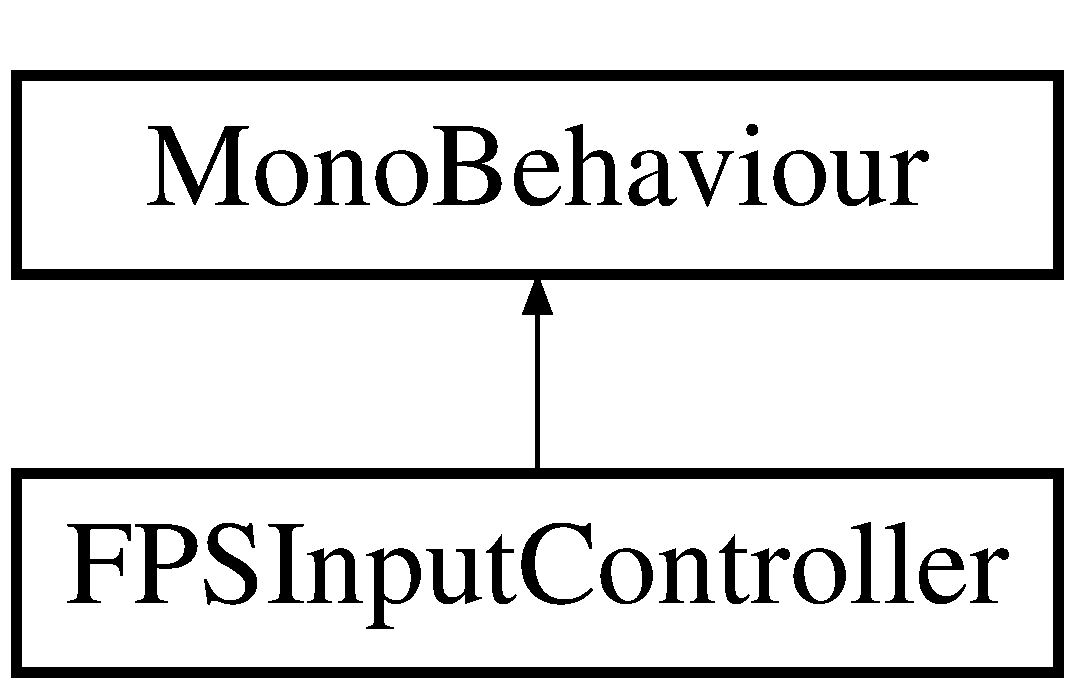
\includegraphics[height=2.000000cm]{class_f_p_s_input_controller}
\end{center}
\end{figure}
\subsection*{Public Attributes}
\begin{DoxyCompactItemize}
\item 
bool \hyperlink{class_f_p_s_input_controller_a9e52965685f8d0253de430b56d0359e9}{check\+Auto\+Walk} = false
\end{DoxyCompactItemize}


\subsection{Member Data Documentation}
\hypertarget{class_f_p_s_input_controller_a9e52965685f8d0253de430b56d0359e9}{}\index{F\+P\+S\+Input\+Controller@{F\+P\+S\+Input\+Controller}!check\+Auto\+Walk@{check\+Auto\+Walk}}
\index{check\+Auto\+Walk@{check\+Auto\+Walk}!F\+P\+S\+Input\+Controller@{F\+P\+S\+Input\+Controller}}
\subsubsection[{check\+Auto\+Walk}]{\setlength{\rightskip}{0pt plus 5cm}bool F\+P\+S\+Input\+Controller.\+check\+Auto\+Walk = false}\label{class_f_p_s_input_controller_a9e52965685f8d0253de430b56d0359e9}


The documentation for this class was generated from the following file\+:\begin{DoxyCompactItemize}
\item 
\hyperlink{_f_p_s_input_controller_8cs}{F\+P\+S\+Input\+Controller.\+cs}\end{DoxyCompactItemize}

\hypertarget{class_load_on_click}{}\section{Load\+On\+Click Class Reference}
\label{class_load_on_click}\index{Load\+On\+Click@{Load\+On\+Click}}
Inheritance diagram for Load\+On\+Click\+:\begin{figure}[H]
\begin{center}
\leavevmode
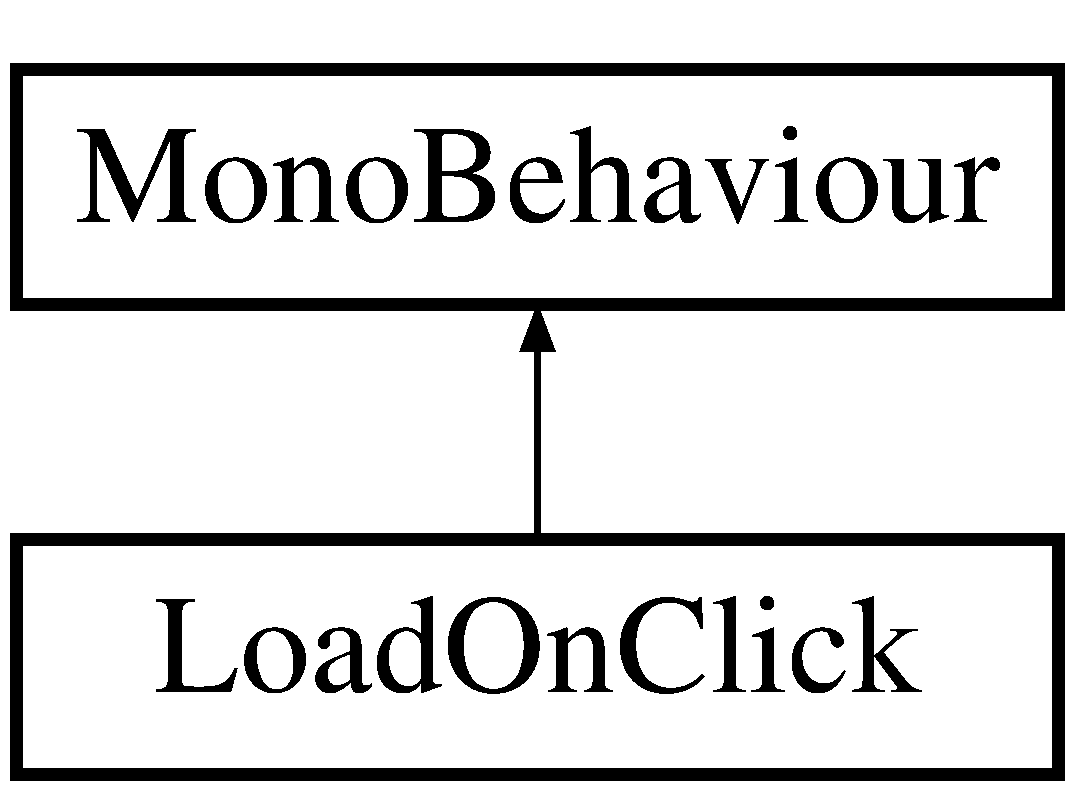
\includegraphics[height=2.000000cm]{class_load_on_click}
\end{center}
\end{figure}
\subsection*{Public Member Functions}
\begin{DoxyCompactItemize}
\item 
void \hyperlink{class_load_on_click_a28cd054e026094a5fa36c4fb9b15b3ba}{Load\+Scene} (string level)
\begin{DoxyCompactList}\small\item\em Main Function used to change scenes. \end{DoxyCompactList}\end{DoxyCompactItemize}
\subsection*{Public Attributes}
\begin{DoxyCompactItemize}
\item 
Game\+Object \hyperlink{class_load_on_click_a9135e1be868b982e1c8ff7242d35e469}{loading\+Image}
\end{DoxyCompactItemize}


\subsection{Member Function Documentation}
\hypertarget{class_load_on_click_a28cd054e026094a5fa36c4fb9b15b3ba}{}\index{Load\+On\+Click@{Load\+On\+Click}!Load\+Scene@{Load\+Scene}}
\index{Load\+Scene@{Load\+Scene}!Load\+On\+Click@{Load\+On\+Click}}
\subsubsection[{Load\+Scene(string level)}]{\setlength{\rightskip}{0pt plus 5cm}void Load\+On\+Click.\+Load\+Scene (
\begin{DoxyParamCaption}
\item[{string}]{level}
\end{DoxyParamCaption}
)}\label{class_load_on_click_a28cd054e026094a5fa36c4fb9b15b3ba}


Main Function used to change scenes. 


\begin{DoxyParams}{Parameters}
{\em String} & level for the scene name \\
\hline
\end{DoxyParams}
\begin{DoxyReturn}{Returns}
Should not return. 
\end{DoxyReturn}


\subsection{Member Data Documentation}
\hypertarget{class_load_on_click_a9135e1be868b982e1c8ff7242d35e469}{}\index{Load\+On\+Click@{Load\+On\+Click}!loading\+Image@{loading\+Image}}
\index{loading\+Image@{loading\+Image}!Load\+On\+Click@{Load\+On\+Click}}
\subsubsection[{loading\+Image}]{\setlength{\rightskip}{0pt plus 5cm}Game\+Object Load\+On\+Click.\+loading\+Image}\label{class_load_on_click_a9135e1be868b982e1c8ff7242d35e469}


The documentation for this class was generated from the following file\+:\begin{DoxyCompactItemize}
\item 
\hyperlink{_load_on_click_8cs}{Load\+On\+Click.\+cs}\end{DoxyCompactItemize}

\chapter{File Documentation}
\hypertarget{_autowalk_8cs}{}\section{Autowalk.\+cs File Reference}
\label{_autowalk_8cs}\index{Autowalk.\+cs@{Autowalk.\+cs}}


This script moves your player automatically in the direction he is looking at.  


\subsection*{Classes}
\begin{DoxyCompactItemize}
\item 
class \hyperlink{class_autowalk}{Autowalk}
\end{DoxyCompactItemize}


\subsection{Detailed Description}
This script moves your player automatically in the direction he is looking at. 

You can activate the autowalk function by pull the cardboard trigger, by define a threshold angle or combine both by selecting both of these options. The threshold is an value in degree between 0° and 90°. So for example the threshold is 30°, the player will move when he is looking 31° down to the bottom and he will not move when the player is looking 29° down to the bottom. This script can easally be configured in the Unity Inspector.\+Attach this Script to your Cardboard\+Main-\/\+Game\+Object. If you haven\textquotesingle{}t the Cardboard Unity S\+D\+K, download it from \href{https://developers.google.com/cardboard/unity/download}{\tt https\+://developers.\+google.\+com/cardboard/unity/download}

\begin{DoxyAuthor}{Author}
Peter Huynh 

Cary Sullivan
\end{DoxyAuthor}
\begin{DoxyRefDesc}{Bug}
\item[\hyperlink{bug__bug000001}{Bug}]Collision isn\textquotesingle{}t handled.\end{DoxyRefDesc}

\hypertarget{_character_motor_8cs}{}\section{Character\+Motor.\+cs File Reference}
\label{_character_motor_8cs}\index{Character\+Motor.\+cs@{Character\+Motor.\+cs}}


Character motor holds all the values for the speed and movement of a 3\+D object within unity and handles collision.  


\subsection*{Classes}
\begin{DoxyCompactItemize}
\item 
class \hyperlink{class_character_motor}{Character\+Motor}
\item 
class \hyperlink{class_character_motor_1_1_character_motor_movement}{Character\+Motor.\+Character\+Motor\+Movement}
\item 
class \hyperlink{class_character_motor_1_1_character_motor_jumping}{Character\+Motor.\+Character\+Motor\+Jumping}
\item 
class \hyperlink{class_character_motor_1_1_character_motor_moving_platform}{Character\+Motor.\+Character\+Motor\+Moving\+Platform}
\item 
class \hyperlink{class_character_motor_1_1_character_motor_sliding}{Character\+Motor.\+Character\+Motor\+Sliding}
\end{DoxyCompactItemize}


\subsection{Detailed Description}
Character motor holds all the values for the speed and movement of a 3\+D object within unity and handles collision. 

\begin{DoxyAuthor}{Author}
Peter Huynh 

Cary Sullivan
\end{DoxyAuthor}
\begin{DoxyRefDesc}{Bug}
\item[\hyperlink{bug__bug000002}{Bug}]Accelerates spontaniously if attached to a camera\end{DoxyRefDesc}

\hypertarget{_f_p_s_input_controller_8cs}{}\section{F\+P\+S\+Input\+Controller.\+cs File Reference}
\label{_f_p_s_input_controller_8cs}\index{F\+P\+S\+Input\+Controller.\+cs@{F\+P\+S\+Input\+Controller.\+cs}}


The controller for the main character that navigates the \hyperlink{class_character_motor}{Character\+Motor} movement properties.  


\subsection*{Classes}
\begin{DoxyCompactItemize}
\item 
class \hyperlink{class_f_p_s_input_controller}{F\+P\+S\+Input\+Controller}
\end{DoxyCompactItemize}


\subsection{Detailed Description}
The controller for the main character that navigates the \hyperlink{class_character_motor}{Character\+Motor} movement properties. 

\begin{DoxyAuthor}{Author}
Peter Huynh 

Cary Sullivan
\end{DoxyAuthor}
\begin{DoxyRefDesc}{Bug}
\item[\hyperlink{bug__bug000003}{Bug}]None\end{DoxyRefDesc}

\hypertarget{_load_on_click_8cs}{}\section{Load\+On\+Click.\+cs File Reference}
\label{_load_on_click_8cs}\index{Load\+On\+Click.\+cs@{Load\+On\+Click.\+cs}}


Class designed to change scenes within the Unity project.  


\subsection*{Classes}
\begin{DoxyCompactItemize}
\item 
class \hyperlink{class_load_on_click}{Load\+On\+Click}
\end{DoxyCompactItemize}


\subsection{Detailed Description}
Class designed to change scenes within the Unity project. 

\begin{DoxyAuthor}{Author}
Peter Huynh 

Cary Sullivan
\end{DoxyAuthor}
\begin{DoxyRefDesc}{Bug}
\item[\hyperlink{bug__bug000004}{Bug}]None\end{DoxyRefDesc}

%--- End generated contents ---

% Index
\backmatter
\newpage
\phantomsection
\clearemptydoublepage
\addcontentsline{toc}{chapter}{Index}
\printindex

\end{document}
